\documentclass[12pt]{article}
\usepackage[utf8]{inputenc}
\usepackage{float}
\usepackage{amsmath}
\usepackage{tikz}
\def\checkmark{\tikz\fill[scale=0.4](0,.35) -- (.25,0) -- (1,.7) -- (.25,.15) -- cycle;}


\usepackage[hmargin=3cm,vmargin=6.0cm]{geometry}
%\topmargin=0cm
\topmargin=-2cm
\addtolength{\textheight}{6.5cm}
\addtolength{\textwidth}{2.0cm}
%\setlength{\leftmargin}{-5cm}
\setlength{\oddsidemargin}{0.0cm}
\setlength{\evensidemargin}{0.0cm}
\setlength{\parskip}{1em}

%misc libraries goes here
%\usepackage{fitch}


\begin{document}

\section*{CENG435 - Term Project Report (Part 1) } 

\section*{Student Information }

Name : Orçun Başşimşek \\
Id Number : 2098804 \\
\\
Name : Murat Doğan \\
Id Number : 2188498 \\

\section{Introduction}

\ \ \ \ In this project, we developed UDP Socket application to find link costs using RTT calculations and conduct an experiment to analyze end-to-end delay for specified nodes on given network topology. For our coding implementations, we preferred Java as programming language. Details are explained in next sections.

\section{Discovery of Link Costs}

\ \ \ \ Before starting implement our approach, we created a slice named "61tp" on GENI platform. Then, we added given "download\textunderscore topology.xml" file to Cenic InstaGENI as our resource. After that, we reached our R1 and R2 nodes and exeucted given "configureR1.sh" and "configureR2.sh" scripts on these nodes respectively.

As mentioned earlier, we preferred Java programming language to implement our approach. We mainly used Java's DatagramSocket class to create our UDP sockets, and DatagramPacket class to send and receive our discovery messages. While sending and receiving messages, we achieved simultaneity with multithreading concepts in Java. In this first part of project, our aim was to find all link's costs by calculating RTT values of each link many times, and average them. We know that, RTT is a required time for a message(or packet) to go from source node to destination and return back to the source again. We firstly thought that for each node, there must be a component that is responsible for only sending discovery messages to all neighbours and getting back an acknowledgement message from these neighbours specifically. We called these components simply as \textbf{Client}. Also, there must be another part that is responsible for only receiving messages from neighbours and returning back an acknowledgement message for each received message specifically. We also called these components simply as \textbf{Server}.

\subsection{Server Implementation}
\ \ \ \ We firstly started with our \textbf{Server} implementations for each node. In our implementation, each node has one Server thread as a main thread. These Server threads just open a DatagramSocket(which accepts UDP protocol) on a specific port. Then, it just starts to listen discovery messages from that port. We did not prefer more than one Server that run on different threads and listen just one specific neighbour. Instead of this approach, we preferred just one Server thread for each node because \textbf{connectionless} nature of UDP protocol. For example, for node S, there is only one Server thread. And, this thread simply listens a specific port (e.g. for our implementation, port 1050 for node S server). After that, all client neighbours of node S (nodes R1-R2-R3 for our case) can send their discovery messages to node S server(port:1050) simultaneously without any connection. Thus, we did not need specific listener Servers that run on different threads for each neighbour Client actually. Of course, with our single threaded server approach, each coming message is handled one by one and then responded. However, in project specifications, it is stated that each node should receive multiple message at the same time, not should handle multiple message at the same time. Besides that, if we preferred different Server threads approach for each neighbour Client specifically, we observed that RTT values were so small and too close to compare. For these reasons, we prefer single thread approach for Server implementations.

Our main Server thread for each node runs as follows in general.(There are some small differences according to our messaging and saving link costs scenario which will be explained later.) It simply expects 1000 discovery messages from each neighbours. (For example server on node D expects 3000 messages since node D has 3 neighbours. However, server on node R2 expects 4000 messages since node R2 has 4 neighbours.) Then, each coming messages are handled one by one. From coming DatagramPacket, source's IP address and port are extracted. Then, a simple string("ACK") is returned back to the source node's Client. One more responsibility of Server codes is starting Client threads which are responsible for sending discovery messages to each neighbours specifically. After handling all receiving messages, server simply is closed.  

\subsection{Client Implementation}
\ \ \ \ As mentioned earlier, we supposed Clients as just discovery message senders to neighbours' Servers. But for this time, it is impossible to send messages to different neighbours simultaneously with single thread. For this time, we definitely needed to different sender Client threads for each of our neighbours. For example, for node S, we needed to 3 Client threads. One of them is responsible for sending message to R1 node, second of them sends messages to R2 node, and third of them sends messages to R3 node at the same time. These client threads are created and started in our main Server thread according to our messaging scenario.     

Our Client threads run as follows in general. Their job is simple: just sending 1000 discovery messages to one specific neighbour. Besides that, RTT calculations of specified link and saving link costs are done in Client threads. For RTT calculations, client saves the time when it sends a message as \textbf{Send Time}. Then, it starts to wait "ACK" feedback from destination node's Server. When Client receives this packet, it also saves this time as \textbf{Receive Time}. And then, it simply calculate RTT for one message as follows: 
\begin{center}
$RTT = Receive \ Time - Send \ Time$
\end{center}
For each of 1000 message, this calculations is repeated, and then their average are considered as \textbf{Link Cost} in our approach. After completing the sending messages, client thread's socket is closed.

\subsection{Messaging Scenario and Saving Link Costs}
\ \ \ \ In our messaging scenario, node S is initiator of messages and node S's script must be ran lastly. When we run each of D-R3-R2-R1 scripts, servers on these nodes stand up and starts to listen receiving messages. When we run node S script lastly, server on node S is also stand up, and node S creates 3 sender Client for each of its neighbour(R1-R2-R3). After that, when first messages are coming to R1-R2-R3 servers from S sender clients, servers on R1-R2-R3 know that messaging is started and these servers create and start their sender clients for each of their neighbours. For example, when R1 server gets first message, then it creates 3 clients for S-R2-D nodes. R2 server creates 4 clients for S-R1-R3-D nodes, and R3 server creates 3 clients for sending messages to S-R2-D nodes. The approach is also similar for node D also. When node D server gets its first message, it also creates its sender client threads for R1-R2-R3 neighbours of D. With this scenario, each node is able to sends messages to their neighbours with its Client threads, and receive messages from neighbours with its Server thread simultaneously. If we specifically think R1-R2 link for example, R1 client thread for R2 sends 1000 messages and get 1000 "ACK" feedbacks, and R2 client thread for R1 sends 1000 messages and get 1000 "ACK" feedbacks. Therefore, total 4000 messages travel on R1-R2 link, and this scenario is same for each link with our approach(Of course packet losses are included in these 4000 messages as a natural thing for UDP).

For saving link costs, we preferred that link costs of R1-S, R1-R2 and R1-D are saved by R1 client threads as "link\textunderscore cost(R1-S).txt", "link\textunderscore cost(R1-R2).txt" and "link\textunderscore cost(R1-D).txt" respectively. Link costs of R2-S, R2-R3 and R2-D are saved by corresponding R2 client threads as "link\textunderscore cost(R2-S).txt", "link\textunderscore cost(R2-R3).txt" and "link\textunderscore cost(R2-D).txt" respectively. And finally, links costs of R3-S and R3-D are saved by corresponding R3 client threads as "link\textunderscore cost(R3-S).txt", "link\textunderscore cost(R3-D).txt" respectively.
    
\section{Finding Shortest Path From Node S to Node D With Dijkstra's Shortest Path Algorithm}
\begin{center}
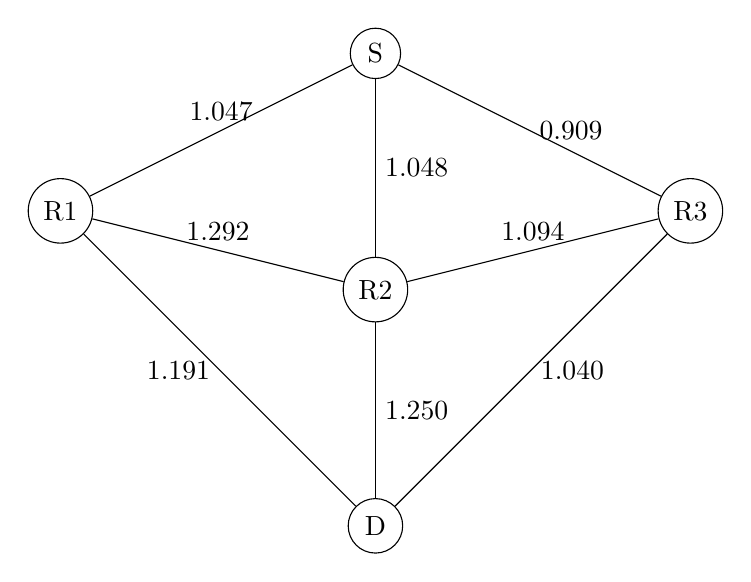
\begin{tikzpicture}
\draw
(5, 7) node[circle, black, draw](s){S}
(1, 5) node[circle, black, draw](r1){R1}
(5, 4) node[circle, black, draw](r2){R2}
(9, 5) node[circle, black, draw](r3){R3}
(5, 1) node[circle, black, draw](d){D};



\draw[-] (s) -- node[above] {1.047} (r1);
\draw[-] (s) -- node[right] {1.048} (r2);
\draw[-] (s) -- node[right] {0.909} (r3);
\draw[-] (r1) -- node[above] {1.292} (r2);
\draw[-] (r1) -- node[left] {1.191} (d);
\draw[-] (r2) -- node[above] {1.094} (r3);
\draw[-] (r2) -- node[right] {1.250} (d);
\draw[-] (r3) -- node[right] {1.040} (d);

\end{tikzpicture}
\end{center}

\begin{center}
\ \ \ \ \ \ \ \ \ \ \ Figure 1: Link costs on given topology. (Costs in milliseconds)
\newline
\vspace*{1 cm}
\newline
\end{center}



\begin{table}[htbp]
  \centering
  \bgroup
  \def\arraystretch{1.5}
  \resizebox{\textwidth}{!}{
    \begin{tabular}{c|c|c|c|c|c}
    Marked     & S     & R1    & R2    & R3 &  D  \\
    \hline
    \hline
    S \checkmark     & \fbox{0}     & $\infty$     & $\infty$     & $\infty$     & $\infty$  \\
    \hline
    R3 \checkmark     & \fbox{0}     & \begin{tabular}{@{}c@{}}Min($\infty$, 0+1.047) \\ 1.047\end{tabular}     & \begin{tabular}{@{}c@{}}Min($\infty$, 0+1.048) \\ 1.048\end{tabular}     & \begin{tabular}{@{}c@{}}Min($\infty$, 0+0.909) \\ \fbox{0.909}\end{tabular}     & $\infty$  \\
    \hline
    R1     & \fbox{0}     & \fbox{1.047}     & \begin{tabular}{@{}c@{}}Min(1.048, 0.909+1.094) \\ 1.048\end{tabular}     & \fbox{0.909}     & \begin{tabular}{@{}c@{}}Min($\infty$, 0.909+1.040) \\ 1.949\end{tabular}  \\
    \hline
    R2     & \fbox{0}     & \fbox{1.047}     & \begin{tabular}{@{}c@{}}Min(1.048, 1.047+1.292) \\ \fbox{1.048}\end{tabular}     & \fbox{0.909}     & \begin{tabular}{@{}c@{}}Min(1.949, 1.047+1.191) \\ 1.949\end{tabular}  \\
    \hline
    D \checkmark     & \fbox{0}     & \fbox{1.047}     & \fbox{1.048}     & \fbox{0.909}     & \begin{tabular}{@{}c@{}}Min(1.949, 1.048+1.250) \\ \fbox{1.949}\end{tabular}  \\
    \hline
    \end{tabular}}
    \egroup
\end{table}%
\begin{center}
Table 1: Shortest path table
\end{center}

After finding all link's costs as in Figure 1, we used Dijkstra's Shortest Path Algorithm to find the shortest distance from node S to node D. For this reason, firstly, we constructed shortest path table(Table 1). Values in the cells, denotes the weight of shortest path from node S to that column's node. For first row, we wrote 0 distance in S column, and infinity distances from S node to corresponding nodes to other columns. After filling first row, we found smallest unmarked value as 0 in S column, and marked it with a square box, and write this node to "Marked" column of first row. Since, value in column S is marked in first row, we looked only direct neighbours of S node in second row. For second row, we copied all marked values from first row(which is just zero for this time). For direct neighbours of marked node, we used following formula to calculate weight of shortest path from source node to corresponding column node:
\begin{center}
$Min(Destination \ Value, \ Marked \ Value + Edge \ Weight) $
\end{center}
Destination value is value of previous row for a specific column. Marked Value is last marked value from previous row, and edge weight is just our link costs. With this formula, column R1-R2-R3 of second row is filled properly. For column D of second row, previous value from previous row is just copied because there is no direct connection between last marked node's column(which is node S) to node D. After filling second row completely, we again marked smallest unmarked value which is 0.909 in R3 column in second row, and wrote this node to "Marked" column of second row. For third row, again we copied all marked values from previous row, and this time we investigated direct neighbours of node R3 since last marked value is in R3 column from previous row. We filled columns R2 and D with our formula. Since there is no direct connection between R1 and R3, R1 value from previous node is just copied. After filling third row completely, we again marked smallest unmarked value which is 1.047 in column R1 for this time, and again wrote it to "Marked" column of third row, and same process continues like this for fourth and fifth rows as well. Finally, the marked value in destination column which is D column in our case is weight of shortest path from node S to node D. It is 1.949 ms as seen in the Table 1.

Now, we found weight of our shortest path as 1.949 ms. To find shortest path, we used backtracking. For this reason, we first ticked node D as destination node in "Marked" column of last row. Then, we move upward one row and checked the value in lastly ticked node's column which is D column. The value in D column is still 1.949 in fourth row, so we continued by moving one row upward. The value in D column for third row is still 1.949, so we continued by moving one row upward. Now in second row, our value in D column changed(it is infinity for second row), so we ticked the node in "Marked" column for second row(which is R3). From now, we considered the changes in lastly ticked node's column(which is 0.909 for R3 column in second row). Then, we moved upward to first row, and value in lastly ticked column(which is R3 column) is again changed to infinity. Thus, we also ticked the node in "Marked" column of first row.

Finally, we collect all ticked nodes in "Marked" column of our shortest path table from up to down. \textbf{Therefore, our shortest path is S-R3-D with weight of 1.949 ms.}

\section{End-to-end Delay Calculations}
\ \ \ \ From now on, we only dealt with S, R3 and D nodes because we needed to calculate end-to-end delay from node S to node D over shortest path. For this reason, we modified our discovery scripts a little bit. We know that end-to-end delay is a required time for a message(or packet) to go from source node to destination node(one way travel). It is different from RTT(which is required time for message to go and back) in discovery part. For this time, in our approach, there is no distinct server-client class implementations in our code. We simply implemented the following scenario. (Of course, we did some synchronization configurations between S and D node's System times, and all of these are explained in our ReadMe file).  Node S sends a message to node R3 and saves the time using Java's System current time in milliseconds method as \textbf{Send Time from node S}. Then this message is transmitted from node R3 to node D. Node D receives this message, and it also saves the time with same approach as \textbf{Receive Time on node D}. Then, node D sends this "receive time" information to node R3, and node R3 delivers this information to node S again. Finally, node S calculates end-to-end delay for this just one message as:
\begin{center}
$End-to-end \ delay = Receive \ Time \ on \ node \ D - Send \ Time \ from \ node \ S$
\end{center}

This process is repeated again for 1000 messages, and finally node S takes the average of these times and finds end-to-end delay from node S to node D over shortest path. As a note, in our implementation, we also included packet losses in our average as we did in RTT calculations at discovery part.

\section{Experiment Results}
\ \ \ \ First of all, we applied step 1, and added $20 \ ms \pm 5 \ ms$ delays to all links of S-R3-D nodes with normal distribution using tc/netem commands (Details of commands are explained in our ReadMe file). Then for this step, we ran our scripts \textbf{5} times and we got average of total \textbf{5000} messages' end-to-end delay as \textbf{43.9 ms}. For second step, we added $40 \ ms \pm 5 \ ms$ delays to all links of S-R3-D nodes, and got  average of total \textbf{5000} messages' end-to-end delay as \textbf{86.7 ms}. Finally, we added $50 \ ms \pm 5 \ ms$ delays to all links of S-R3-D nodes, and got average of total \textbf{5000} messages' end-to-end delay as \textbf{107.1 ms}.

Then, we applied \textbf{\%95 confidence interval} to these results. Since we chose a very large sample size(total 5000 messages), we calculated confidence interval according to results of 5 running of scripts, and take the sample size as 5 for simplicity. \\
\\
\\
\\
\\
\\
Hence, our results are: \\
For Step 1: $43.9 \pm 0.369 \ ms$ \\
For Step 2: $86.7 \pm 2.65 \ ms$ \\
For Step 3: $107.1 \pm 3.11 \ ms$ \\

\begin{figure}[h!]
  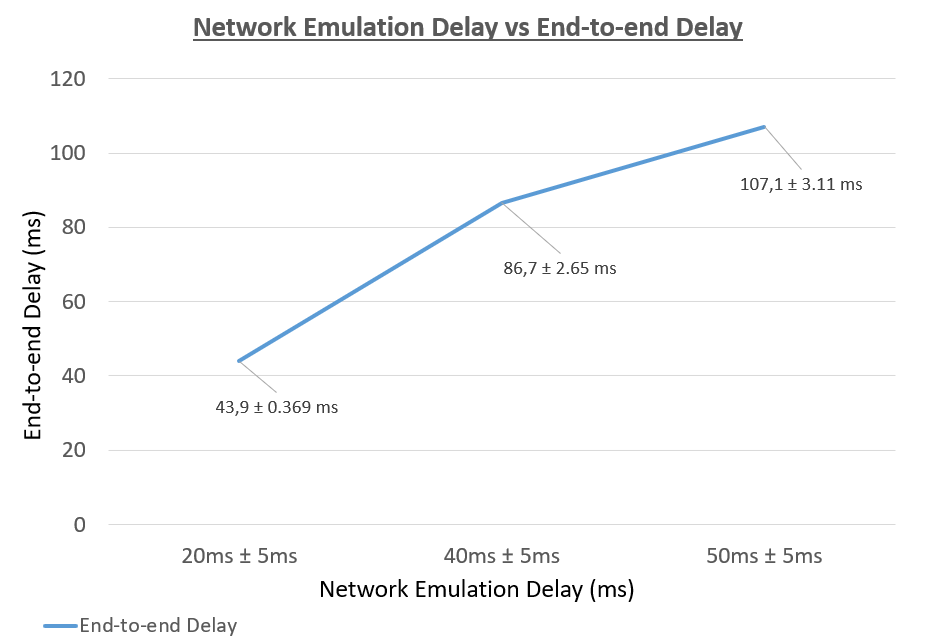
\includegraphics[width=\linewidth]{435graph.png}
\end{figure}


We observed that our results are consistent with our RTT calculations. We found the shortest path as S-R3-D as mentioned earlier. While calculation of end-to-end delay from node S to node D among this path, it is expected that result will be the sum of end-to-end delay from node S to node R3 and end-to-end delay from node R3 to node D. In our results, while applying $20 \ ms \pm 5 \ ms$ delay to all links of (S-R3-D), end-to-end delay is approximately $2* (20 \ ms \pm 5 \ ms)$ as expected. Again for second step, end-to-end delay is approximately $2* (40 \ ms \pm 5 \ ms)$ as expected. For third step, same scenario happened.

  


\end{document}

​

